% ---------------------------------------------------------------------------
% FiLM-TCN model section.
%
% Packages assumed in the preamble: amsmath, amssymb, booktabs, natbib,
% graphicx. Figure~\ref{fig:filmtcn} includes figures/filmtcn_arch.pdf,
% compiled from paper/figures/filmtcn_arch.tex (TikZ, standalone).
% Citation keys: perez2018film (already in your .bib); the others are in
% paper/filmtcn_refs.bib -- rename them if your .bib uses different keys.
% Every equation, dimension and default below follows models/ModernTCN.py,
% data_provider/ and the colab_benchmark_h1_h5.ipynb configuration
% (--use_events --event_fusion channel --event_dim 16, shared embedding).
% ---------------------------------------------------------------------------
\providecommand{\FiLMTCN}{FiLM-TCN}

\subsection{FiLM-TCN}
\label{sec:filmtcn}

\FiLMTCN{} uses FiLM to condition a ModernTCN representation of past
volatility on the macroeconomic announcements scheduled for the forecast
horizon. The model treats covariates according to when they are known.
Covariates observed only up to day $t$ (in our application, the announcement
calendar over the look-back window) form an additional variable: they are
embedded, patched with the same patch length and stride as the target series,
and pass through the ModernTCN blocks, where the variable-mixing layer lets
them interact with the target. Only the known future
covariates, the announcement calendar for the forecast horizon, enter through
FiLM.

The FiLM layer is also placed differently from the original design. Instead of
modulating every block, as \citet{perez2018film} do, we apply a single FiLM
layer to the output of the final ModernTCN block. The backbone therefore
encodes the history, past announcements included, without reference to the
forecast-horizon calendar, and that calendar acts only on the finished
representation. In our experiments this placement gave better forecasts than
FiLM layers inside each block.
Section~\ref{sec:dummies-to-film} shows what this conditioning adds relative
to announcement dummies in a HAR regression. Figure~\ref{fig:filmtcn} shows
the architecture.

\begin{figure}[tbp]
  \centering
  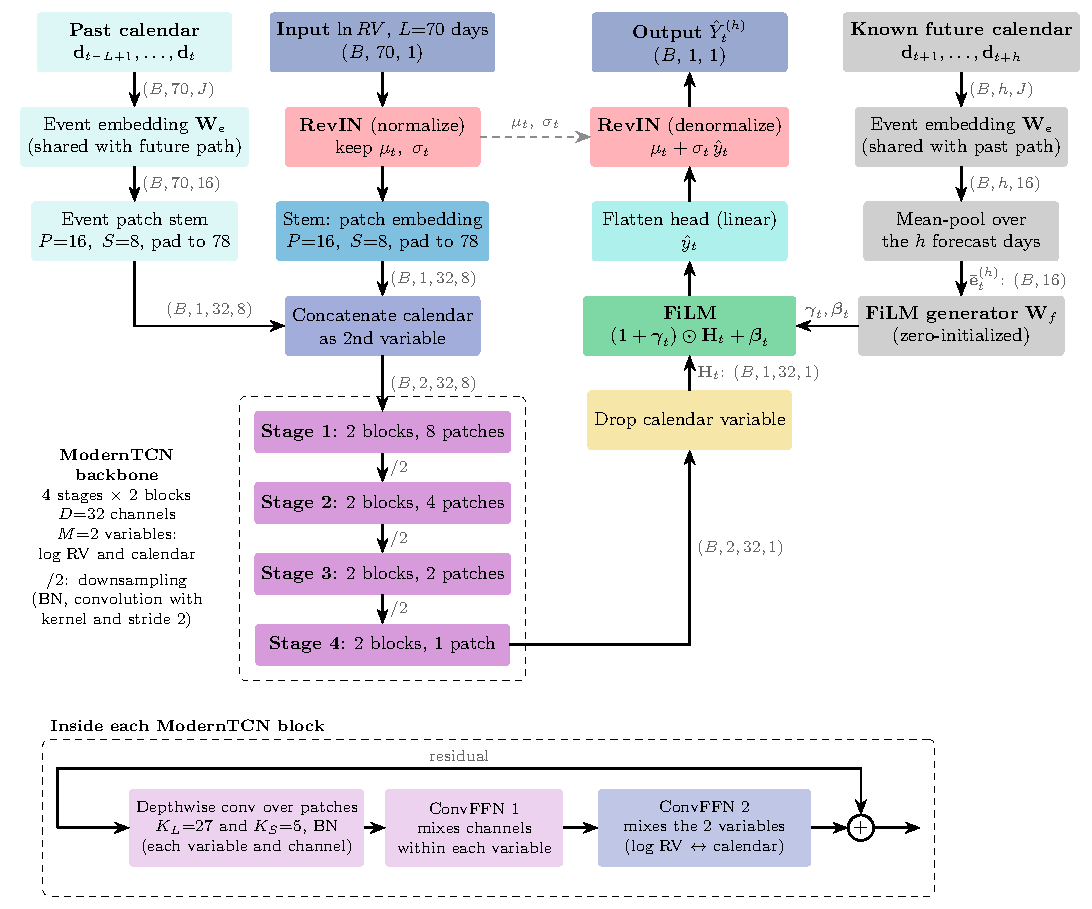
\includegraphics[width=\textwidth]{figures/filmtcn_arch}
  \caption{\FiLMTCN{} as estimated in this paper. The look-back calendar is
    embedded, patched by its own stem and concatenated with log realized
    variance as a second variable; both variables pass through four ModernTCN
    stages, and the calendar variable is dropped after the last one. The
    forecast-horizon calendar is embedded with the same $\mathbf{W}_e$,
    averaged over the $h$ forecast days and mapped to the FiLM parameters
    $\boldsymbol{\gamma}_t$ and $\boldsymbol{\beta}_t$, which rescale and
    shift the history representation $\mathbf{H}_t$ before the linear head.
    Both stems pad the 70-day window at its end to 78 days, which gives
    $N=8$ patches. Grey labels on the arrows give tensor shapes, as
    (batch, days, features) before the mean-pool and as (batch, variables,
    channels, patches) inside the backbone, or name the quantity passed;
    $/2$ marks downsampling. $J$ is the number of calendar features.}
  \label{fig:filmtcn}
\end{figure}

\subsubsection{Inputs and forecast target}
\label{sec:filmtcn-inputs}

Let $x_s = \ln RV_s$ denote log realized variance on trading day $s$, $t$ the
forecast origin and $h$ the horizon in trading days. At every horizon the model
forecasts the log of realized variance averaged over the forecast window,
\begin{equation}
  Y_t^{(h)}
  = \ln\Bigl(\frac{1}{h}\sum_{k=1}^{h} RV_{t+k}\Bigr)
  = \ln\sum_{k=1}^{h} e^{x_{t+k}} - \ln h ,
  \label{eq:filmtcn-target}
\end{equation}
which equals $x_{t+1}$ when $h=1$. The value input is the look-back window
$\mathbf{x}_t = (x_{t-L+1},\dots,x_t)^\top$ of $L$ trading days.

% If the data section already defines the calendar, replace this paragraph
% with a reference to it and keep only the last two sentences.
Announcements enter through a daily calendar vector
$\mathbf{d}_s \in \mathbb{R}^{J}$. Its first three entries count the releases
scheduled on day $s$, in total and for each of the two currencies of the pair;
they are standardized with the mean and standard deviation of the training
years. The remaining entries are indicators $D_{j,s}\in\{0,1\}$, one for each
release type $j$ that is scheduled on at least 24 trading days, equal to one
when $j$ is scheduled on day $s$. The 24 days are counted over the full sample,
12 January 2012 to 30 June 2025, so the selection of release types also sees
the validation and test years. A release dated on a non-trading day is
assigned to the next trading day. This gives $J = 253$ for AUD/USD, $322$ for
EUR/USD and $270$ for GBP/USD. The model reads the calendar over two windows:
the look-back days, $\mathbf{d}_{t-L+1},\dots,\mathbf{d}_t$, and the forecast
days, $\mathbf{d}_{t+1},\dots,\mathbf{d}_{t+h}$. The second window is known at
$t$ because release dates are published in advance. It records only that an
announcement is scheduled, never its outcome.

\subsubsection{Normalization and patch embedding}
\label{sec:filmtcn-embedding}

Following \citet{kim2022revin}, each value window is normalized with its own
moments,
\begin{equation}
  \mu_t = \frac{1}{L}\sum_{i=0}^{L-1} x_{t-i}, \qquad
  \sigma_t = \Bigl(\frac{1}{L}\sum_{i=0}^{L-1}(x_{t-i}-\mu_t)^2
             + \epsilon\Bigr)^{1/2}, \qquad
  \tilde{x}_s = \frac{x_s-\mu_t}{\sigma_t},
  \label{eq:filmtcn-revin}
\end{equation}
with $\epsilon = 10^{-5}$, and the forecast is mapped back to the log-variance
scale with the same $\mu_t$ and $\sigma_t$ in~\eqref{eq:filmtcn-output}. We use
RevIN without its learnable affine parameters. The calendar is not normalized
in this way.

The normalized window is split into overlapping patches of length $P$ taken
every $S$ days. We pad the end of the window with $P-S$ copies of
$\tilde{x}_t$, which gives $N = \lfloor L/S \rfloor$ patches,
\begin{equation}
  \tilde{\mathbf{p}}_{t,n}
  = (\tilde{x}_{\tau_n+1},\dots,\tilde{x}_{\tau_n+P})^\top,
  \qquad \tau_n = t-L+(n-1)S, \qquad n = 1,\dots,N,
  \label{eq:filmtcn-patch}
\end{equation}
where $\tilde{x}_s = \tilde{x}_t$ for $s>t$. A stem maps each patch to $D$
channels,
\begin{equation}
  \mathbf{z}^{x}_{t,n}
  = \operatorname{BN}\bigl(\mathbf{W}_x\tilde{\mathbf{p}}_{t,n}
    + \mathbf{b}_x\bigr) \in \mathbb{R}^{D},
  \qquad \mathbf{W}_x \in \mathbb{R}^{D\times P},
  \label{eq:filmtcn-stem-x}
\end{equation}
where $\operatorname{BN}$ denotes batch normalization. This is a
one-dimensional convolution with kernel size $P$ and stride $S$.

Before patching, the calendar of each day is embedded linearly,
\begin{equation}
  \mathbf{e}_s = \mathbf{W}_e\mathbf{d}_s + \mathbf{b}_e \in \mathbb{R}^{d_e},
  \qquad \mathbf{W}_e \in \mathbb{R}^{d_e\times J}.
  \label{eq:filmtcn-embed}
\end{equation}
Since most entries of $\mathbf{d}_s$ are indicators, $\mathbf{e}_s$ is the sum
of the embeddings (the columns of $\mathbf{W}_e$) of the release types scheduled
on day $s$, plus the count terms and the intercept $\mathbf{b}_e$. The embedded
look-back calendar is padded and patched with the geometry
of~\eqref{eq:filmtcn-patch}, setting $\mathbf{e}_s = \mathbf{e}_t$ for $s>t$,
and passed through a stem of its own,
\begin{equation}
  \mathbf{z}^{d}_{t,n}
  = \operatorname{BN}\Bigl(\sum_{p=1}^{P}\mathbf{W}_{d,p}\,\mathbf{e}_{\tau_n+p}
    + \mathbf{b}_d\Bigr) \in \mathbb{R}^{D},
  \qquad \mathbf{W}_{d,p} \in \mathbb{R}^{D\times d_e}.
  \label{eq:filmtcn-stem-d}
\end{equation}
Stacking the two gives the input to the backbone,
$\mathbf{Z}^{(0)}_t \in \mathbb{R}^{M\times D\times N}$ with $M=2$: variable
$m=1$ holds $\mathbf{z}^{x}_{t,1},\dots,\mathbf{z}^{x}_{t,N}$ and variable $m=2$
holds $\mathbf{z}^{d}_{t,1},\dots,\mathbf{z}^{d}_{t,N}$. The calendar is
therefore one additional variable rather than $J$ of them, because the
embedding~\eqref{eq:filmtcn-embed} compresses the $J$ calendar series to $d_e$
before patching.

\subsubsection{ModernTCN backbone}
\label{sec:filmtcn-backbone}

The backbone stacks the residual blocks of \citet{luo2024moderntcn}. Write the
input of a block as $\mathbf{Z}\in\mathbb{R}^{M\times D\times N}$ with entries
$z_{m,c,n}$ for variable $m$, channel $c$ and patch $n$; a dot in place of an
index denotes the vector along that axis. A block computes
\begin{align}
  \mathbf{u}_{m,c,\cdot}
    &= \operatorname{BN}\bigl(\mathbf{k}_{m,c} * \mathbf{z}_{m,c,\cdot}\bigr)
     + \operatorname{BN}\bigl(\mathbf{k}'_{m,c} * \mathbf{z}_{m,c,\cdot}\bigr),
     \label{eq:filmtcn-dw}\\
  \bar{\mathbf{u}}_{m,\cdot,n}
    &= \operatorname{BN}\bigl(\mathbf{u}_{m,\cdot,n}\bigr),
     \label{eq:filmtcn-dw-norm}\\
  \mathbf{v}_{m,\cdot,n}
    &= \mathbf{W}^{(2)}_{m}\operatorname{GELU}\bigl(\mathbf{W}^{(1)}_{m}
       \bar{\mathbf{u}}_{m,\cdot,n} + \mathbf{b}^{(1)}_{m}\bigr)
     + \mathbf{b}^{(2)}_{m},
     \label{eq:filmtcn-ffn1}\\
  \mathbf{o}_{\cdot,c,n}
    &= \mathbf{W}^{(4)}_{c}\operatorname{GELU}\bigl(\mathbf{W}^{(3)}_{c}
       \mathbf{v}_{\cdot,c,n} + \mathbf{b}^{(3)}_{c}\bigr)
     + \mathbf{b}^{(4)}_{c},
     \label{eq:filmtcn-ffn2}\\
  \mathbf{Z} &\leftarrow \mathbf{Z} + \mathbf{O}.
     \label{eq:filmtcn-residual}
\end{align}
In~\eqref{eq:filmtcn-dw}, $*$ is a one-dimensional convolution over patches,
zero-padded to keep $N$ patches, and each variable--channel pair has its own
large kernel $\mathbf{k}_{m,c}\in\mathbb{R}^{K_L}$ and small kernel
$\mathbf{k}'_{m,c}\in\mathbb{R}^{K_S}$. The batch normalization
in~\eqref{eq:filmtcn-dw-norm} pools the statistics of each channel over the two
variables. The first feed-forward layer~\eqref{eq:filmtcn-ffn1} mixes channels
within a variable, with $\mathbf{W}^{(1)}_m\in\mathbb{R}^{rD\times D}$ and
$\mathbf{W}^{(2)}_m\in\mathbb{R}^{D\times rD}$. The second
layer~\eqref{eq:filmtcn-ffn2} mixes variables within a channel, with
$\mathbf{W}^{(3)}_c\in\mathbb{R}^{rM\times M}$ and
$\mathbf{W}^{(4)}_c\in\mathbb{R}^{M\times rM}$. During training, dropout is
applied after each of the four pointwise maps.

The three operations act on different axes: the depthwise convolution mixes
patches within a variable and channel, the first feed-forward layer mixes
channels within a variable, and the second mixes variables. With $M=2$,
\eqref{eq:filmtcn-ffn2} is therefore the only operation in which the volatility
variable and the calendar variable exchange information. It does so in every
block: for each channel and patch, the update of the volatility feature is a
small network of that feature and the corresponding calendar feature.

The blocks are arranged in $G$ stages of $n_b$ blocks each. Before every stage
after the first, each variable passes through a batch normalization and a
convolution with kernel size and stride $2$, which halves the number of
patches; its weights are shared by the two variables. After the last stage the
calendar variable is discarded, and the representation of the history is
\begin{equation}
  \mathbf{H}_t = \bigl(h_{t,c,n}\bigr)
  = \bigl(z^{(G)}_{1,c,n}\bigr) \in \mathbb{R}^{D\times N_G},
  \label{eq:filmtcn-history}
\end{equation}
where $N_G = \lceil N/2^{G-1}\rceil$ (when a stage receives an odd number of
patches, the last patch is repeated before downsampling). In our configuration
(Table~\ref{tab:filmtcn-hparams}) the four stages see $8$, $4$, $2$ and $1$
patches, so $\mathbf{H}_t$ is a single vector of $D=32$ channels.
$\mathbf{H}_t$ depends on the values and the calendar of the look-back window
only.

\subsubsection{Conditioning on the forecast-horizon calendar}
\label{sec:filmtcn-film}

The forecast-horizon calendar is summarized by the mean of its daily
embeddings,
\begin{equation}
  \bar{\mathbf{e}}^{(h)}_t
  = \frac{1}{h}\sum_{k=1}^{h}\mathbf{e}_{t+k}
  = \mathbf{W}_e\,\bar{\mathbf{d}}^{(h)}_t + \mathbf{b}_e,
  \qquad
  \bar{\mathbf{d}}^{(h)}_t = \frac{1}{h}\sum_{k=1}^{h}\mathbf{d}_{t+k},
  \label{eq:filmtcn-cond}
\end{equation}
where $\mathbf{W}_e$ and $\mathbf{b}_e$ are the embedding
of~\eqref{eq:filmtcn-embed}, shared with the look-back calendar. For an
indicator entry, $\bar{d}^{(h)}_{t,j}$ is the share of the $h$ forecast days on
which release type $j$ is scheduled, which is how the announcement regressors
of the HAR regression in Section~\ref{sec:dummies-to-film} are constructed.

A linear generator maps the summary to a scale and a shift for each channel,
\begin{equation}
  \begin{pmatrix}\boldsymbol{\gamma}_t\\ \boldsymbol{\beta}_t\end{pmatrix}
  = \mathbf{W}_f\,\bar{\mathbf{e}}^{(h)}_t + \mathbf{b}_f,
  \qquad
  \mathbf{W}_f \in \mathbb{R}^{2D\times d_e},\quad
  \mathbf{b}_f \in \mathbb{R}^{2D},
  \label{eq:filmtcn-generator}
\end{equation}
and the FiLM layer modulates the representation of the history,
\begin{equation}
  \hat{h}_{t,c,n} = (1+\gamma_{t,c})\,h_{t,c,n} + \beta_{t,c},
  \qquad c = 1,\dots,D,\quad n = 1,\dots,N_G.
  \label{eq:filmtcn-film}
\end{equation}
Every channel is rescaled and shifted by an amount set by the calendar, and the
same amount applies to every patch. We parameterize the scale as
$1+\gamma_{t,c}$ and initialize $\mathbf{W}_f$ and $\mathbf{b}_f$ at zero, so
that at initialization the FiLM layer is the identity and the network forecasts
from the backbone alone. The generator has $2D(d_e+1) = 1{,}088$ parameters.

A linear head reads the modulated representation, and the RevIN moments
of~\eqref{eq:filmtcn-revin} return the forecast to the log-variance scale,
\begin{equation}
  \hat{y}_t = b_h + \sum_{c=1}^{D}\sum_{n=1}^{N_G} w_{c,n}\,\hat{h}_{t,c,n},
  \qquad
  \hat{Y}^{(h)}_t = \mu_t + \sigma_t\,\hat{y}_t .
  \label{eq:filmtcn-output}
\end{equation}
The model produces one number per origin, the forecast of $Y^{(h)}_t$
in~\eqref{eq:filmtcn-target}, at every horizon. During training, the output of
the head passes through dropout with rate 0.134: with that probability
$\hat{y}_t$ is set to zero, so that the forecast equals $\mu_t$, and otherwise
it is scaled by $1/(1-0.134)$.

\subsubsection{What the conditioning computes}
\label{sec:filmtcn-decomposition}

Because the head is linear and the FiLM layer is affine, the forecast can be
written in closed form given $\mathbf{H}_t$. Substituting~\eqref{eq:filmtcn-film}
into~\eqref{eq:filmtcn-output} gives
\begin{equation}
  \hat{Y}^{(h)}_t
  = \mu_t + \sigma_t\bigl(\hat{y}^{0}_t
    + \boldsymbol{\omega}^\top\boldsymbol{\beta}_t
    + \mathbf{g}_t^\top\boldsymbol{\gamma}_t\bigr),
  \label{eq:filmtcn-decomp}
\end{equation}
where $\hat{y}^{0}_t = b_h + \sum_{c,n} w_{c,n}h_{t,c,n}$ is the normalized
forecast with the FiLM layer removed, $\omega_c = \sum_n w_{c,n}$, and
$g_{t,c} = \sum_n w_{c,n}h_{t,c,n}$ is the head's reading of channel $c$ of the
history. The shift $\boldsymbol{\beta}_t$ moves the forecast additively, while
the scale $\boldsymbol{\gamma}_t$ acts through its product with the history.

Split the generator into its scale and shift rows,
$\mathbf{W}_f = (\mathbf{W}_\gamma^\top, \mathbf{W}_\beta^\top)^\top$ and
$\mathbf{b}_f = (\mathbf{b}_\gamma^\top, \mathbf{b}_\beta^\top)^\top$.
By~\eqref{eq:filmtcn-cond}, both are affine in the horizon calendar,
\begin{equation}
  \boldsymbol{\gamma}_t = \mathbf{A}_\gamma\bar{\mathbf{d}}^{(h)}_t
    + \boldsymbol{\gamma}_0,
  \qquad
  \boldsymbol{\beta}_t = \mathbf{A}_\beta\bar{\mathbf{d}}^{(h)}_t
    + \boldsymbol{\beta}_0,
  \label{eq:filmtcn-loadings}
\end{equation}
with loadings
$\mathbf{A}_\gamma = \mathbf{W}_\gamma\mathbf{W}_e$ and
$\mathbf{A}_\beta = \mathbf{W}_\beta\mathbf{W}_e$ in
$\mathbb{R}^{D\times J}$ and intercepts
$\boldsymbol{\gamma}_0 = \mathbf{W}_\gamma\mathbf{b}_e + \mathbf{b}_\gamma$
and $\boldsymbol{\beta}_0 = \mathbf{W}_\beta\mathbf{b}_e + \mathbf{b}_\beta$.
The effect of release type $j$ on the forecast is then
\begin{equation}
  \frac{\partial\hat{Y}^{(h)}_t}{\partial\bar{d}^{(h)}_{t,j}}
  = \sigma_t\bigl(\boldsymbol{\omega}^\top\mathbf{a}_{\beta,j}
    + \mathbf{g}_t^\top\mathbf{a}_{\gamma,j}\bigr),
  \label{eq:filmtcn-effect}
\end{equation}
where $\mathbf{a}_{\beta,j}$ and $\mathbf{a}_{\gamma,j}$ are the $j$-th columns
of $\mathbf{A}_\beta$ and $\mathbf{A}_\gamma$.

Equation~\eqref{eq:filmtcn-effect} makes four properties of the conditioning
explicit. First, inside the parentheses the effect of a release has a part that
is the same at every origin, $\boldsymbol{\omega}^\top\mathbf{a}_{\beta,j}$, and
a part that varies with the recent history through $\mathbf{g}_t$. Second, the
whole effect is scaled by $\sigma_t$, the dispersion of log realized variance in
the look-back window, because the FiLM layer acts before the RevIN moments are
restored: for a given value of the term in parentheses, an announcement moves
the forecast further when log realized variance was more dispersed over the
look-back window. Third, $\mathbf{A}_\gamma$ and $\mathbf{A}_\beta$ factor
through $\mathbf{W}_e$, so their rank is at most $d_e = 16$, against $J$
between 253 and 322 calendar features. Release types do not receive free
coefficients, as in a dummy regression; their effects are read from a shared
$d_e$-dimensional embedding. Fourth, holding $\mathbf{H}_t$ fixed, the forecast
is affine in $\bar{\mathbf{d}}^{(h)}_t$. The effects of two releases scheduled
in the same window therefore add up, with no interaction term, and for $h>1$
the forecast does not depend on which day of the window a release falls on. All nonlinearity
in~\eqref{eq:filmtcn-decomp} comes from the history.

\subsubsection{Estimation}
\label{sec:filmtcn-estimation}

All parameters $\theta$ are estimated jointly, separately for each currency
pair and horizon, by minimizing the mean squared error
\begin{equation}
  \mathcal{L}(\theta)
  = \frac{1}{|\mathcal{T}|}\sum_{t\in\mathcal{T}}
    \bigl(\hat{Y}^{(h)}_t - Y^{(h)}_t\bigr)^2
  \label{eq:filmtcn-loss}
\end{equation}
over the forecast origins $\mathcal{T}$ of the training years. All three series
start on 12 January 2012, so with $L=70$ the first training origin is
19 April 2012. The last training origin is the latest one whose $h$-day target
window ends by 31 December 2021: 30 December 2021 at $h=1$ and 24 December 2021
at $h=5$. This gives 2,515 training origins at $h=1$ and 2,511 at $h=5$. Each epoch draws shuffled mini-batches of 256 origins
and drops the last incomplete batch, so it uses 9 batches, or 2,304 origins.

We use Adam \citep{kingma2015adam} without weight decay and a one-cycle
learning-rate schedule \citep{smith2019superconvergence}, updated after every
mini-batch and planned over the maximum of 40 epochs. With the PyTorch defaults
we keep, the rate rises from $2.5\times10^{-4}$ to its peak of
$6.35\times10^{-3}$ over the first 30\% of that budget, that is, by the end of
epoch 12, and then decays by cosine annealing; Adam's $\beta_1$ moves from 0.95
to 0.85 and back over the same cycle. Training stops when the validation loss
over 2022--2023 has not improved for 8 epochs, and we keep the parameters with
the lowest validation loss. Because the schedule is fixed in advance, a run
that stops before epoch 12 never reaches the peak rate. The validation loss is
computed on two shuffled batches of 256 origins, 512 of the 514--519
validation origins. Each configuration is trained with the seeds
$2021,\dots,2030$, and the losses we report are averages over seeds.

Table~\ref{tab:filmtcn-hparams} lists the hyperparameters. The look-back
length, the network dimensions, the dropout rates, the learning rate and the
batch size are the optimum of an Optuna search \citep{akiba2019optuna} for
ModernTCN on EUR/USD at $h=1$ [state the EUR/USD series and sample the search
used]. The search held the optimizer and the one-cycle schedule fixed and
trained each trial for at most 30 epochs with patience 7. We raise the dropout
rate in the blocks from the optimum of 0.33 to 0.5. The search has no calendar
embedding, so $d_e=16$ is set separately [state how $d_e=16$ was chosen].
% Candidate, if this is how d_e was chosen: tuningresults/EVENTTCN1 searched
% d_e in {4, 8, 16} for the event model at h = 1 and selected 16 (EVENTTCN5
% selected 4 at h = 5, EVENTTCN22 selected 8 at h = 22). That search used a
% different backbone (seq_len 22, patch 32, 3 blocks). E.g.: "We take d_e = 16
% from a second search, for FiLM-TCN at h = 1 over d_e in {4, 8, 16}; none of
% its other values are used."
All values are held fixed across pairs and horizons. The ModernTCN benchmark
is the same network with the calendar variable and the FiLM layer removed
($M=1$), trained with the same hyperparameters and seeds. Because \FiLMTCN{}
creates its calendar layers before the backbone, a given seed does not give the
two networks the same initial backbone weights or the same batch order, so the
difference between the two models isolates the calendar path only on average
over seeds.

\begin{table}[t]
  \centering
  \caption{\FiLMTCN{} hyperparameters. The ModernTCN benchmark uses the same
    values without the calendar embedding.}
  \label{tab:filmtcn-hparams}
  \begin{tabular}{llr}
    \toprule
    & Symbol & Value \\
    \midrule
    Look-back length                    & $L$            & 70 \\
    Patch length, stride                & $P$, $S$       & 16, 8 \\
    Patches entering the first stage    & $N$            & 8 \\
    Stages, blocks per stage            & $G$, $n_b$     & 4, 2 \\
    Channels                            & $D$            & 32 \\
    Feed-forward expansion ratio        & $r$            & 2 \\
    Depthwise kernel sizes              & $K_L$, $K_S$   & 27, 5 \\
    Calendar embedding dimension        & $d_e$          & 16 \\
    Calendar features (AUD, EUR, GBP)   & $J$            & 253, 322, 270 \\
    Dropout in blocks, in head          &                & 0.5, 0.134 \\
    Batch size                          &                & 256 \\
    Peak learning rate                  &                & $6.35\times10^{-3}$ \\
    Maximum epochs, patience            &                & 40, 8 \\
    Random seeds                        &                & 2021--2030 \\
    \bottomrule
  \end{tabular}
\end{table}
